\documentclass[12pt]{article}
\usepackage[spanish,es-noshorthands,es-tabla]{babel}
\usepackage[T1]{fontenc}
\usepackage[utf8]{inputenc}
\usepackage{newtxtext,newtxmath}   % Times New Roman, as required by the journal
\usepackage[letterpaper,top=2.5cm,bottom=2.5cm,left=3cm,right=3cm]{geometry}
\usepackage{graphicx,booktabs,amsmath,hyperref,xcolor,float}
\usepackage[nocompress]{cite}
\usepackage[skip=4pt]{caption}
\captionsetup[figure]{position=top}
\captionsetup[table]{position=top}
\newcommand{\fuente}{\par\vspace{2pt}{\footnotesize Fuente: elaboración propia.}}
\setlength{\parindent}{0pt}
\setlength{\parskip}{6pt}
\graphicspath{{figures/}}
\hypersetup{colorlinks=true,linkcolor=black,citecolor=black,urlcolor=blue}



\begin{document}
\sloppy
\begin{flushright}
{\LARGE\bfseries Benchmarking AI-generated parallel C++ code: 2D image convolution with OpenMP\par}
\vspace{10pt}
{\Large Benchmarking de código C++ paralelo generado por inteligencia artificial: convolución 2D de imágenes con OpenMP\par}
\end{flushright}
\vspace{14pt}
\ifdefined\versionciega
\begin{center}
{\large Versión para revisión ciega: autores y afiliación omitidos.\par}
\end{center}
\else
\begin{center}
{\large Esteban David Muñoz Bautista \quad Isabela Gutierrez Reyes\par}
\vspace{6pt}
Pontificia Universidad Javeriana Cali, Facultad de Ingeniería\\
Carrera de Ingeniería de Sistemas y Computación\\
\texttt{estebanmunoz13@javerianacali.edu.co}\\
\texttt{isabelagutierrez@javerianacali.edu.co}
\end{center}
\fi

\section*{Abstract}
\textbf{Objective:} to quantify the effect of parallelization on a C++ 2D convolution and compare AI-generated and human-written parallel code.
\textbf{Methods and materials:} four variants were evaluated: sequential, parallel generated directly by AI (Claude Opus 5.5), AI-generated with team-directed optimization, and an OpenMP implementation from a 2016 public repository. Images from 512² to 4096² pixels, 3×3 to 11×11 kernels and 1--16 threads were used, with 30 runs per configuration and bit-exact validation against the sequential version.
\textbf{Results and discussion:} on 4096² images the AI variant reached speedups of 36.9--61.8 over the sequential code, except for 11×11 (12.7), where it lost vectorization; the directed optimization raised it to 48.0. The human implementation, a direct (naive) parallelization, reached 5.8--6.7. Scalability relative to one thread was similar for all variants (6--10 at 16 threads).
\textbf{Conclusions:} the AI code was correct on the first attempt and, through vectorization, much faster than the human implementation, but showed a data-dependent weakness that only measurement revealed. Future work should evaluate other AI models, an expert-optimized manual implementation and other architectures.

\textbf{Keywords:} parallel programming; OpenMP; 2D convolution; AI-generated code; benchmarking; speedup.

\section*{Resumen}
\textbf{Objetivo:} cuantificar el efecto de la paralelización en una convolución 2D en C++ y comparar código paralelo generado por inteligencia artificial (IA) y escrito por personas.
\textbf{Materiales y métodos:} se evaluaron cuatro variantes: secuencial, generada directamente por IA (Claude Opus 5.5), de IA con optimización dirigida por el equipo y una implementación OpenMP pública de 2016. Se usaron imágenes de 512² a 4096² píxeles, kernels de 3×3 a 11×11 y de 1 a 16 hilos, con 30 repeticiones por configuración y verificación bit a bit contra la versión secuencial.
\textbf{Resultados y discusión:} en 4096² la variante de IA alcanzó speedups de 36,9 a 61,8 frente a la secuencial, salvo con 11×11 (12,7), donde perdió su vectorización; la optimización dirigida lo elevó a 48,0. La implementación humana, una paralelización directa (naive), logró entre 5,8 y 6,7. La escalabilidad respecto a un hilo fue similar (6 a 10 con 16 hilos).
\textbf{Conclusiones:} el código de IA fue correcto al primer intento y, por vectorización, mucho más rápido que la implementación humana, pero mostró una debilidad dependiente de los datos que solo reveló la medición. Como trabajo futuro se propone evaluar otros modelos de IA, una implementación manual optimizada y otras arquitecturas.

\textbf{Palabras clave:} programación paralela; OpenMP; convolución 2D; código generado por IA; benchmarking; speedup.

\section{Introducción}
Los asistentes de programación basados en modelos de lenguaje generan hoy código funcional en lenguajes de alto rendimiento \cite{chen2021codex}. Estudios recientes han evaluado su capacidad para producir núcleos paralelos con OpenMP, CUDA y otros modelos de programación, principalmente en términos de corrección y, en menor medida, de rendimiento \cite{godoy2023,nichols2024}. Para un ingeniero, la pregunta práctica no es solo si el código compila y es correcto, sino cuánto rendimiento entrega frente a una implementación escrita por personas y frente a la versión secuencial.

Este trabajo estudia esa pregunta con un núcleo clásico de procesamiento de imágenes: la convolución 2D \cite{gonzalez2018}. El objetivo general es determinar cuantitativamente el impacto de la paralelización sobre el rendimiento de código C++ generado por IA, bajo condiciones idénticas de hardware, software, imágenes de entrada y parámetros de convolución. Los objetivos específicos son: (i) medir tiempo de ejecución, speedup, eficiencia y desviación estándar de cuatro variantes; (ii) analizar su escalabilidad con 1 a 16 hilos; (iii) comparar el código generado directamente por IA, el código de IA optimizado bajo dirección del equipo y una implementación paralela escrita por personas; y (iv) verificar la equivalencia funcional estricta de todas las variantes. El estudio evalúa el código tal como lo produce cada fuente: en el caso de la IA se mide su capacidad combinada de aplicar paralelismo multihilo y optimizaciones por núcleo (como la vectorización), no solo su uso de OpenMP. Para separar ambos efectos se reportan métricas referidas a la versión secuencial y a la propia variante con un hilo.

\section{Materiales y métodos}

\subsection{Entorno de hardware y software}
Todas las mediciones se realizaron en una sola máquina, descrita en la Tabla~\ref{tab:entorno}. Los datos se registraron automáticamente con un script incluido en el repositorio. No se fijó afinidad de hilos ni política de espera de OpenMP (variables \texttt{OMP\_PROC\_BIND} y \texttt{OMP\_WAIT\_POLICY} sin definir), de modo que se midió el comportamiento por defecto del runtime.

\begin{table}[H]
\centering
\caption{Entorno experimental.}
\label{tab:entorno}
\begin{tabular}{lp{11cm}}
\toprule
Componente & Valor \\
\midrule
CPU & Intel Core i7-10700F, 2,90 GHz, 8 núcleos físicos, 16 hilos lógicos (HyperThreading) \\
Caché & L2 2 MiB, L3 16 MiB \\
Memoria & 32 GB \\
Sistema operativo & Windows 10 Pro 10.0.19045 \\
Compilador & GCC 16.2.0 (WinLibs, MinGW-w64 x86\_64, UCRT, hilos POSIX) \cite{gccdoc} \\
Flags & \texttt{-O2 -fopenmp -std=c++17 -static} (sin \texttt{-march=native} ni \texttt{-ffast-math}) \\
Plan de energía & Perfil personalizado de alto rendimiento \\
Análisis & Python 3.12.6, NumPy 2.1.3, Matplotlib 3.9.2 \\
\bottomrule
\end{tabular}
\fuente
\end{table}

\subsection{Problema y contrato funcional}
Sea $I$ una imagen en escala de grises de $w \times h$ píxeles de 8 bits y $K$ un kernel cuadrado de $k \times k$ pesos enteros no negativos, con $r = \lfloor k/2 \rfloor$. Para cada píxel se calcula
\begin{equation}
A(x,y) = \sum_{i=0}^{k-1} \sum_{j=0}^{k-1} I(y+i-r,\; x+j-r)\, K(i,j),
\label{eq:conv}
\end{equation}
con $I = 0$ fuera de la imagen (zero-padding), acumulando en enteros de 32 bits. La salida es
\begin{equation}
O(x,y) = \min\!\left(255,\; \max\!\left(0,\; \left\lfloor \frac{A(x,y) + \lfloor S/2 \rfloor}{S} \right\rfloor\right)\right), \qquad S = \sum_{i,j} K(i,j).
\label{eq:norm}
\end{equation}
Se usaron kernels binomiales (aproximación entera de un filtro gaussiano), construidos como el producto exterior de la fila $k$ del triángulo de Pascal. Para $k = 11$ la suma es $S = 2^{20}$ y el peso máximo es $252^2 = 63\,504$; el acumulador máximo, $255 \cdot 2^{20} \approx 2{,}7 \times 10^8$, cabe en un entero de 32 bits. Como la suma de enteros es asociativa y conmutativa, el resultado no depende del orden de acumulación; esto permite exigir igualdad bit a bit entre variantes, a diferencia de una implementación en punto flotante.

Las imágenes se generan en memoria con un generador pseudoaleatorio xorshift de 32 bits con semilla fija ($42 + n$ para una imagen de $n \times n$). El costo de la convolución no depende del contenido de la imagen, por lo que las imágenes sintéticas no sesgan el tiempo medido y garantizan reproducibilidad.

\subsection{Variantes evaluadas}
Las cuatro variantes implementan la misma firma \texttt{convolve(in, out, w, h, k, ksize, nthreads)}.

\textbf{Secuencial.} Cuatro bucles anidados que aplican directamente (\ref{eq:conv}) y (\ref{eq:norm}) con verificación de límites; es la referencia de corrección y de tiempo.

\textbf{IA directa.} Se entregó a Claude Opus 5.5 (Anthropic), en una sesión nueva y sin acceso al repositorio, un prompt fijo que describe la firma, la semántica exacta, los flags de compilación, los tamaños y los conteos de hilos, y pide optimizar para CPU x86-64 multinúcleo. El código devuelto se usó sin modificaciones. El prompt y la respuesta completos están en el directorio \texttt{ai\_log/} del repositorio. La IA produjo, al primer intento, una versión con reparto estático de filas por hilo, un búfer circular de filas convertidas a enteros de 16 bits y vectorización manual con instrucciones SSE2 (\texttt{\_mm\_madd\_epi16}) \cite{intelintrinsics}. Esta vectorización solo se activa si todos los pesos caben en un entero de 16 bits con signo ($\le 32\,767$); en caso contrario usa un camino escalar.

\textbf{IA + optimización dirigida por el equipo.} A partir del análisis del código anterior y de una medición exploratoria, se propusieron cuatro optimizaciones: (O1) mantener la ruta SIMD con pesos de hasta 16 bits sin signo descomponiendo cada peso como $256\,h + l$ con $h, l \le 255$, y combinar $A = 256\,A_h + A_l$; (O2) convolución separable; (O3) AVX2 con despacho en tiempo de ejecución; (O4) una limpieza que elimina una advertencia del compilador. El equipo aprobó O1 y O4 y rechazó O2, porque cambia el algoritmo (de $k^2$ a $2k$ productos por píxel) y rompe la comparabilidad, y O3, porque usaría un conjunto de instrucciones no disponible para las demás variantes con los mismos flags. La implementación de los cambios aprobados se hizo con asistencia de IA; las decisiones están registradas en el repositorio.

\textbf{Manual (GitHub).} Se tomó el método \texttt{Convolutionmp::Compute} del repositorio público \texttt{rdb987/2DConvolution} (commit \texttt{d5b3922}, marzo de 2016) \cite{rdb987}. Se eligió por ser anterior a la disponibilidad de asistentes de código basados en modelos de lenguaje, lo que hace verosímil su autoría humana, y por usar aritmética entera, kernels de tamaño arbitrario y solo OpenMP. Se adaptó lo mínimo: firma común, zero-padding en lugar de bordes periódicos, normalización (\ref{eq:norm}) con un acumulador local por píxel (el original sumaba directamente sobre el arreglo de salida) y \texttt{num\_threads(nthreads)}. Se conservaron su bucle aplanado sobre todos los píxeles (con división y módulo para obtener fila y columna) y su \texttt{\#pragma omp for} con planificación por defecto. Las adaptaciones están documentadas en un diff en el repositorio. Esta implementación es una paralelización directa y no aplica optimizaciones de bajo nivel.

\subsection{Protocolo de medición}
Se evaluaron 4 tamaños ($512^2$, $1024^2$, $2048^2$, $4096^2$), 4 kernels ($3\times3$, $5\times5$, $7\times7$, $11\times11$) y 5 conteos de hilos ($p \in \{1, 2, 4, 8, 16\}$). La variante secuencial se midió solo con $p = 1$. En total hubo 256 configuraciones y 7\,680 mediciones. Para cada configuración y variante:
\begin{enumerate}
\item Se ejecutó una vez sobre un búfer de salida previamente llenado con el valor \texttt{0xAB} y se comparó byte a byte con la salida secuencial; cualquier diferencia aborta el experimento.
\item Se ejecutó una vez más como calentamiento, descartando el tiempo.
\item Se realizaron 30 ejecuciones medidas con \texttt{std::chrono::steady\_clock}, tomando el tiempo exclusivamente alrededor de la llamada a \texttt{convolve} (sin generación de datos, E/S ni validación).
\end{enumerate}
El orden de las variantes se rotó en cada configuración para repartir efectos de calentamiento térmico y de caché.

Además del experimento principal se realizaron dos experimentos complementarios. (i) Sensibilidad a los flags: todas las variantes se recompilaron con \texttt{-O3 -march=native} (que habilita AVX2 en este procesador) y se repitió el protocolo completo para $4096^2$ (64 configuraciones, 1\,920 mediciones). (ii) Anclaje de hilos: se repitieron 12 configuraciones con 8 hilos ($1024^2$ y $2048^2$, kernels de 5 y 11, tres variantes paralelas) con \texttt{OMP\_PROC\_BIND=close} y \texttt{OMP\_PLACES=cores}. Antes del experimento se ejecutó una batería de pruebas automáticas de equivalencia: 5 formas de imagen (incluidas $1\times1$, $5\times3$ ---más pequeña que el kernel--- y formas no cuadradas), los 4 kernels y 6 conteos de hilos (incluido $p = 16$ con solo 3 filas), además de un kernel identidad $1\times1$ y una imagen saturada. Todas las variantes superaron la batería y las 256 validaciones del benchmark.

\subsection{Métricas}
Para cada configuración con $n = 30$ tiempos $t_1, \dots, t_n$ se calculan la media, la desviación estándar muestral y el coeficiente de variación:
\begin{equation}
\bar{T} = \frac{1}{n}\sum_{i=1}^{n} t_i, \qquad \sigma = \sqrt{\frac{1}{n-1}\sum_{i=1}^{n} (t_i - \bar{T})^2}, \qquad CV = \frac{\sigma}{\bar{T}}.
\label{eq:stats}
\end{equation}
El speedup y la eficiencia se calculan como
\begin{equation}
S_p = \frac{T_{seq}}{T_p}, \qquad E_p = \frac{S_p}{p},
\label{eq:speedup}
\end{equation}
donde $T_{seq}$ es el tiempo medio de la variante secuencial (el $T_1$ de la definición clásica) y $T_p$ el tiempo medio de la variante evaluada con $p$ hilos. Como una variante paralela puede ser más rápida que la secuencial incluso con un hilo (por ejemplo, por vectorización), también se reporta el speedup relativo $S^{rel}_p = T^{(v)}_1 / T^{(v)}_p$, que usa el tiempo de la misma variante con un hilo y aísla la escalabilidad por hilos \cite{amdahl1967,gustafson1988,hoefler2015}. Así, $S_p$ combina la ganancia por eficiencia de cada núcleo (incluida la vectorización) con la ganancia por hilos, mientras que $S^{rel}_p$ mide solo la segunda. Por la misma razón, $E_p$ puede ser mayor que 1, y la eficiencia paralela en el sentido clásico es
\begin{equation}
E^{rel}_p = \frac{S^{rel}_p}{p},
\label{eq:erel}
\end{equation}
que vale como máximo 1 en ausencia de efectos superlineales.

Para decidir si dos variantes difieren, se aplicó la prueba U de Mann-Whitney bilateral (aproximación normal con corrección por empates y continuidad) a las 30 mediciones de cada una, con nivel de significancia $\alpha = 0{,}05$. Se eligió una prueba no paramétrica porque los tiempos no tienen por qué seguir una distribución normal. Como se hicieron 80 comparaciones, también se reporta el número de diferencias que siguen siendo significativas con la corrección de Bonferroni ($\alpha/80$). Además del promedio se reporta la mediana, que es menos sensible a ejecuciones atípicas.

\section{Resultados y discusión}
La Tabla~\ref{tab:resumen} resume, para cada imagen y kernel, el tiempo secuencial y el mayor speedup $S_p$ alcanzado por cada variante paralela, con el número de hilos en que se obtuvo. La tabla completa de $4096^2$ (tiempo medio $\pm \sigma$, $S_p$ y $E_p$ para cada $p$) está en el Anexo~\ref{anexo}; las de los demás tamaños y el CSV con las 7\,680 mediciones están en el repositorio.

\begin{table}[H]
\centering
\caption{Tiempo secuencial y mayor speedup $S_p$ por variante (entre paréntesis, hilos en que se obtuvo).}
\label{tab:resumen}
\small
\begin{tabular}{llrrrr}
\toprule
Imagen & Kernel & $T_{seq}$ (ms) & IA directa & IA + opt. equipo & Manual (GitHub) \\
\midrule
512$\times$512 & 3$\times$3 & 2.50 & 19.56 (16) & 19.64 (16) & 5.00 (16) \\
512$\times$512 & 5$\times$5 & 5.35 & 34.66 (16) & 35.52 (8) & 6.24 (16) \\
512$\times$512 & 7$\times$7 & 9.36 & 35.30 (16) & 45.91 (8) & 4.82 (8) \\
512$\times$512 & 11$\times$11 & 21.99 & 13.20 (8) & 47.02 (8) & 6.04 (8) \\
1024$\times$1024 & 3$\times$3 & 10.10 & 22.88 (16) & 23.23 (16) & 4.60 (16) \\
1024$\times$1024 & 5$\times$5 & 21.53 & 50.63 (16) & 50.67 (16) & 6.52 (16) \\
1024$\times$1024 & 7$\times$7 & 37.34 & 64.84 (16) & 54.87 (16) & 6.62 (16) \\
1024$\times$1024 & 11$\times$11 & 87.94 & 11.75 (8) & 54.68 (16) & 6.27 (16) \\
2048$\times$2048 & 3$\times$3 & 39.92 & 37.14 (16) & 37.72 (16) & 5.98 (16) \\
2048$\times$2048 & 5$\times$5 & 86.83 & 52.15 (16) & 54.30 (16) & 6.69 (16) \\
2048$\times$2048 & 7$\times$7 & 150.55 & 67.68 (16) & 66.13 (16) & 6.88 (16) \\
2048$\times$2048 & 11$\times$11 & 351.98 & 15.04 (16) & 57.44 (16) & 6.90 (16) \\
4096$\times$4096 & 3$\times$3 & 162.56 & 36.89 (16) & 36.66 (16) & 6.17 (16) \\
4096$\times$4096 & 5$\times$5 & 344.52 & 56.01 (16) & 57.06 (16) & 6.73 (16) \\
4096$\times$4096 & 7$\times$7 & 597.69 & 61.76 (8) & 58.37 (8) & 6.74 (16) \\
4096$\times$4096 & 11$\times$11 & 1429.85 & 12.70 (16) & 47.95 (16) & 5.79 (16) \\
\bottomrule
\end{tabular}

\fuente
\end{table}

En $4096^2$, la variante secuencial tardó 162,6, 344,5, 597,7 y 1\,429,8 ms con kernels de 3, 5, 7 y 11, respectivamente. Con un solo hilo, la variante de IA directa ya fue 4,7, 7,2 y 8,9 veces más rápida que la secuencial con kernels de 3, 5 y 7, pero solo 2,0 veces con $11\times11$. Con 16 hilos alcanzó $S_{16}$ = 36,9, 56,0, 55,5 y 12,7. La variante con optimización dirigida se comportó igual que la de IA directa en 3, 5 y 7 (diferencias menores que la variabilidad medida), y en $11\times11$ redujo el tiempo de un hilo de 710,7 a 182,9 ms y el de 16 hilos de 112,5 a 29,8 ms ($S_{16} = 48{,}0$). La implementación humana fue más lenta que la secuencial con un hilo ($S_1$ entre 0,64 y 0,81) y alcanzó $S_{16}$ entre 5,8 y 6,7. La Figura~\ref{fig:speedup} muestra $S_p$ y la Figura~\ref{fig:tiempo}, los tiempos con su desviación estándar.

\begin{figure}[H]
\centering
\caption{Speedup $S_p = T_{seq}/T_p$ en imágenes de $4096^2$. La línea punteada es el speedup ideal $S_p = p$; la línea vertical marca $p = 8$ (núcleos físicos).}
\label{fig:speedup}
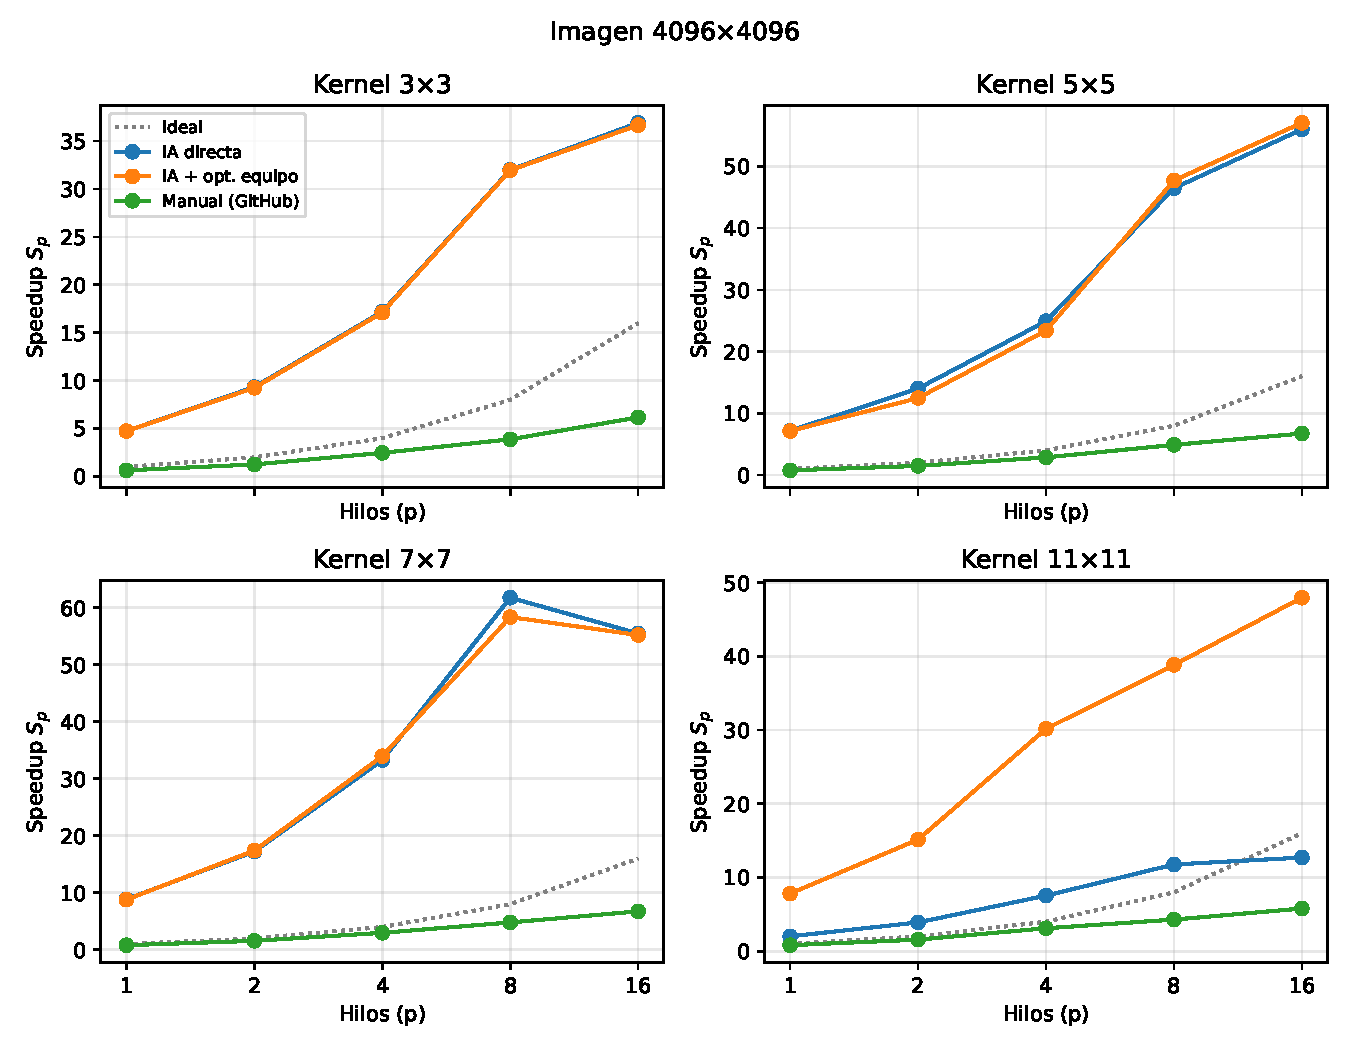
\includegraphics[width=0.85\linewidth]{speedup_4096.pdf}
\fuente
\end{figure}

\begin{figure}[H]
\centering
\caption{Tiempo medio con barras de $\pm\sigma$ en imágenes de $4096^2$ (eje vertical en escala logarítmica). La línea discontinua es el tiempo secuencial.}
\label{fig:tiempo}
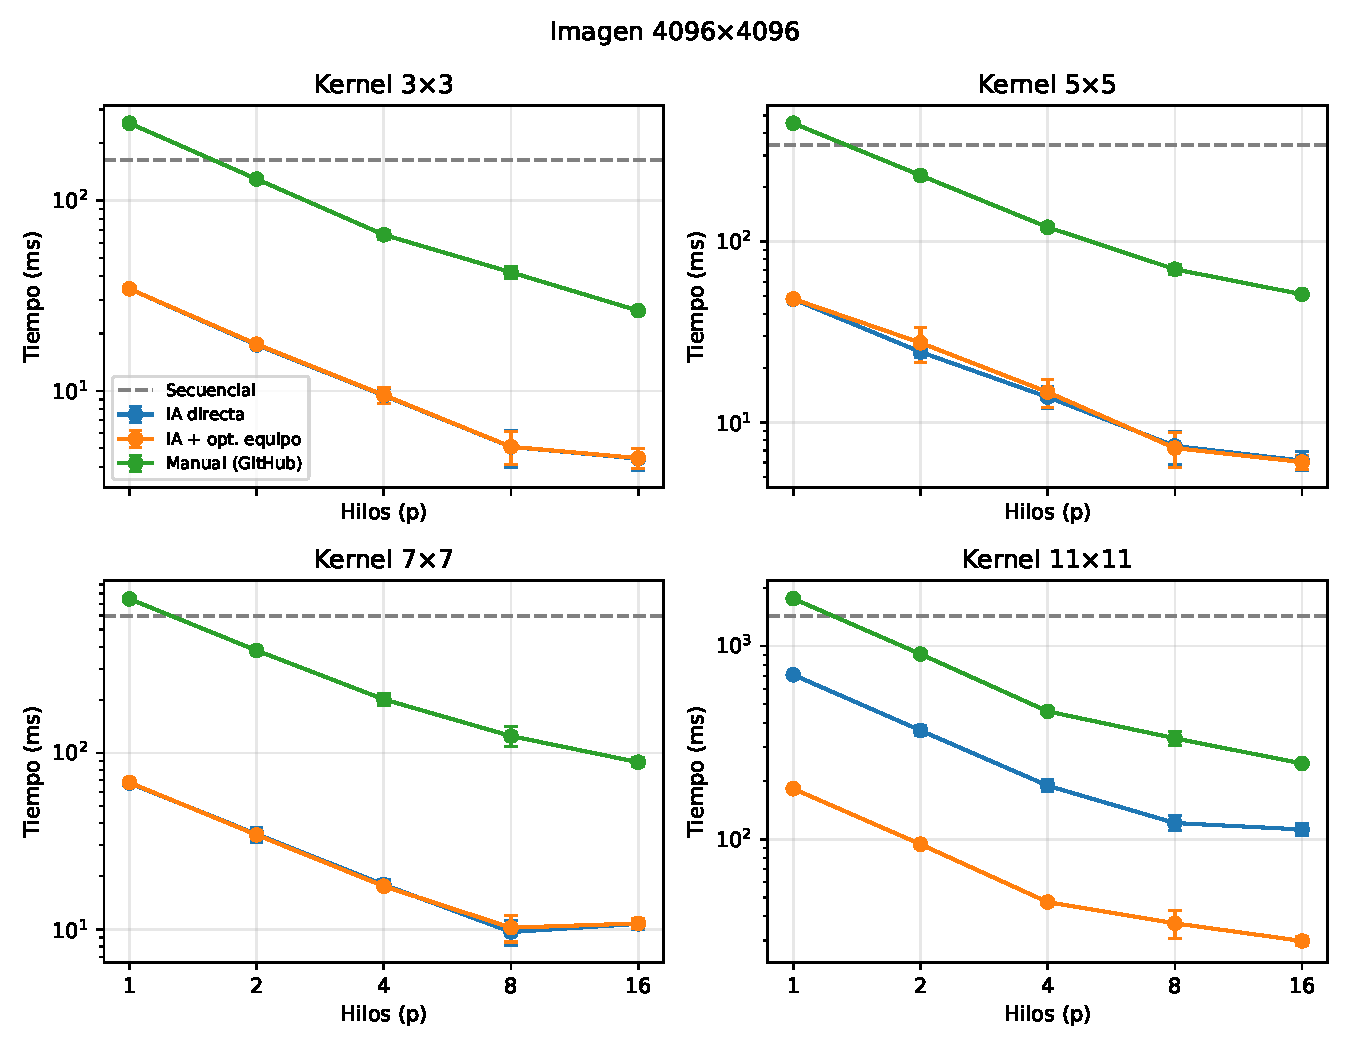
\includegraphics[width=0.85\linewidth]{tiempo_4096.pdf}
\fuente
\end{figure}

La Figura~\ref{fig:relativo} muestra la escalabilidad respecto a cada variante con un hilo. Hasta 4 hilos las tres variantes están cerca del ideal ($S^{rel}_4$ entre 3,3 y 3,9). Con 8 hilos se ubicaron entre 5,0 y 7,0, y con 16 entre 6,1 y 9,6. La variante humana obtuvo el mayor speedup relativo con 16 hilos en los cuatro kernels (7,1 a 9,6 frente a 6,1 a 8,0 de las variantes de IA). Con $7\times7$ en $4096^2$, las variantes de IA fueron más lentas con 16 hilos que con 8 (10,8 frente a 9,7 ms en la variante de IA directa).

\begin{figure}[H]
\centering
\caption{Speedup relativo $T^{(v)}_1/T^{(v)}_p$ de cada variante en imágenes de $4096^2$. La línea vertical marca $p = 8$ (núcleos físicos).}
\label{fig:relativo}
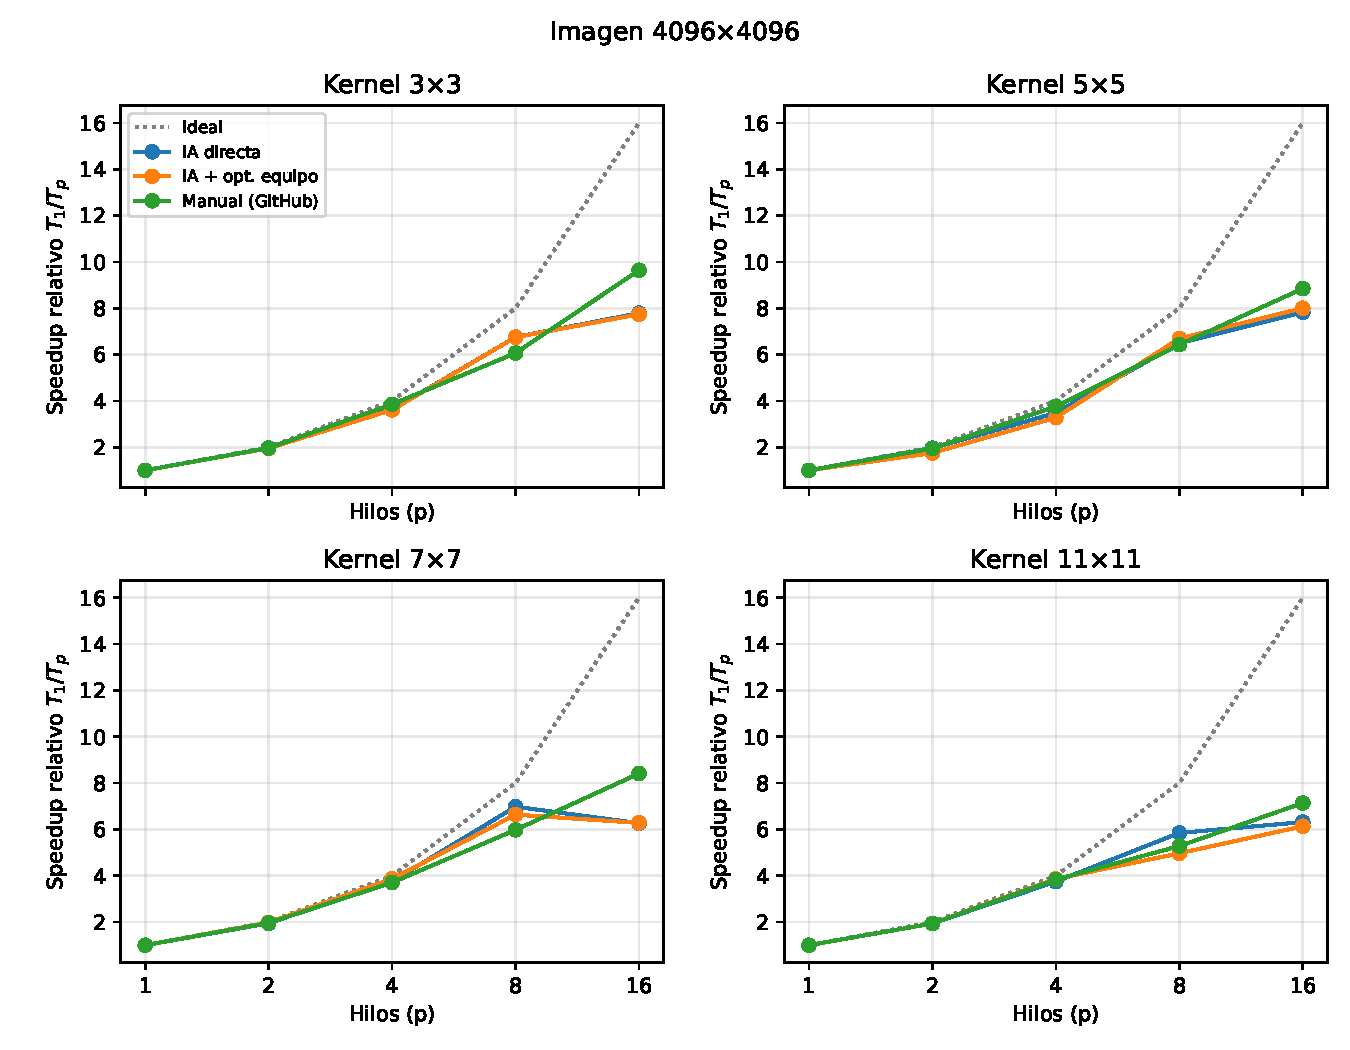
\includegraphics[width=0.85\linewidth]{speedup_relativo_4096.pdf}
\fuente
\end{figure}

La eficiencia respecto a la secuencial (Anexo~\ref{anexo}) es mayor que 1 en las variantes de IA, porque su ventaja con un hilo es mayor que 1, y disminuye con $p$: en $4096^2$ con $11\times11$, $E_{16}$ = 0,79 (IA directa), 3,00 (IA + optimización) y 0,36 (manual). La eficiencia paralela clásica $E^{rel}_p$ (\ref{eq:erel}) separa este efecto: en $4096^2$, con 8 hilos fue de 0,62 a 0,87 en las variantes de IA y de 0,66 a 0,80 en la manual; con 16 hilos bajó a 0,38--0,50 y 0,45--0,60, respectivamente.

Si el speedup se calcula con medianas en lugar de medias, la diferencia típica es de 1,3~\%; solo 21 de las 240 configuraciones paralelas difieren más de un 10~\%, todas con tiempos medios menores que 30 ms. En $4096^2$ con 16 hilos ninguna conclusión cambia (por ejemplo, IA directa con $3\times3$: 36,9 con medias y 39,2 con medianas).

En cuanto a la variabilidad, el $CV$ medio fue 1,2~\% con 1 hilo, 5,0~\% con 2, 9,1~\% con 4, 16,5~\% con 8 y 9,4~\% con 16. En 78 de las 256 configuraciones el $CV$ superó el 10~\%; el grupo más numeroso (36) corresponde a 8 hilos, y 59 de ellas tienen tiempos medios menores que 10 ms. En la variante secuencial el $CV$ no superó el 6,2~\%.

\textbf{Comparación estadística entre IA directa e IA + optimización.} La prueba de Mann-Whitney encontró diferencias significativas en las 20 configuraciones con kernel $11\times11$ ($p < 10^{-4}$ en todas), con medianas entre 3,2 y 5,9 veces menores para la variante optimizada, salvo con 8 hilos en $1024^2$ (1,8 veces). Con kernels de 3, 5 y 7, donde ambas variantes ejecutan casi el mismo código (solo cambia la forma de almacenar los pesos, por O4), 25 de 60 comparaciones fueron significativas con $\alpha = 0{,}05$, pero en ambas direcciones (10 a favor de la variante optimizada y 15 a favor de la de IA directa) y con diferencias de mediana menores que el 7~\% en 20 de ellas. Con la corrección de Bonferroni siguen siendo significativas las 20 comparaciones de $11\times11$ y 11 de las 60 restantes; estas 11 también aparecen en ambas direcciones (5 y 6) y, salvo una, con diferencias de mediana entre 0,5 y 10~\%. La excepción ($512^2$, $7\times7$, 8 hilos: 0,18 frente a 0,29 ms) corresponde a tiempos de décimas de milisegundo.

\textbf{Sensibilidad a los flags de compilación.} La Tabla~\ref{tab:sensibilidad} compara el experimento principal con la recompilación con \texttt{-O3 -march=native} en $4096^2$. El tiempo de la variante secuencial cambió menos del 1~\%: el informe de vectorización de GCC (\texttt{-fopt-info-vec}) muestra que con estos flags solo se vectoriza el bucle que suma los pesos del kernel, no la convolución, en las variantes secuencial y manual. Considerando todos los conteos de hilos, la variante manual cambió entre $-5$~\% y $+10$~\%. En las variantes de IA el efecto dependió del número de hilos: con 1 y 16 hilos (los casos de la tabla) mejoraron entre 2 y 15~\% en la mayoría de los casos, salvo con $7\times7$ y 16 hilos, donde empeoraron cerca de un 20~\%; con 4 y 8 hilos algunas configuraciones fueron hasta un 37~\% más lentas. Las variantes de IA siguieron siendo más rápidas que la manual en todas las configuraciones; en cambio, el orden entre IA directa e IA + optimización en kernels de 3, 5 y 7 cambió en varias configuraciones, lo que es coherente con que sus diferencias sean pequeñas.

\begin{table}[H]
\centering
\caption{Sensibilidad a los flags de compilación en $4096^2$: tiempo medio con \texttt{-O2} (experimento principal) y con \texttt{-O3 -march=native}, y speedup $S_p$ correspondiente.}
\label{tab:sensibilidad}
\small
\begin{tabular}{lrrrrrrr}
\toprule
Variante & Kernel & $p$ & $\bar{T}_{O2}$ (ms) & $\bar{T}_{O3}$ (ms) & $\bar{T}_{O3}/\bar{T}_{O2}$ & $S_p^{O2}$ & $S_p^{O3}$ \\
\midrule
Secuencial & 3 & 1 & 162.56 & 162.48 & 1.00 & 1.00 & 1.00 \\
Secuencial & 5 & 1 & 344.52 & 346.08 & 1.00 & 1.00 & 1.00 \\
Secuencial & 7 & 1 & 597.69 & 595.58 & 1.00 & 1.00 & 1.00 \\
Secuencial & 11 & 1 & 1429.85 & 1416.86 & 0.99 & 1.00 & 1.00 \\
IA directa & 3 & 1 & 34.31 & 30.62 & 0.89 & 4.74 & 5.31 \\
IA directa & 3 & 16 & 4.41 & 3.87 & 0.88 & 36.89 & 41.98 \\
IA directa & 5 & 1 & 48.13 & 43.81 & 0.91 & 7.16 & 7.90 \\
IA directa & 5 & 16 & 6.15 & 5.61 & 0.91 & 56.01 & 61.74 \\
IA directa & 7 & 1 & 67.51 & 62.06 & 0.92 & 8.85 & 9.60 \\
IA directa & 7 & 16 & 10.77 & 13.02 & 1.21 & 55.49 & 45.73 \\
IA directa & 11 & 1 & 710.73 & 695.65 & 0.98 & 2.01 & 2.04 \\
IA directa & 11 & 16 & 112.55 & 108.63 & 0.97 & 12.70 & 13.04 \\
IA + opt. equipo & 3 & 1 & 34.32 & 30.61 & 0.89 & 4.74 & 5.31 \\
IA + opt. equipo & 3 & 16 & 4.43 & 3.75 & 0.85 & 36.66 & 43.32 \\
IA + opt. equipo & 5 & 1 & 48.30 & 42.97 & 0.89 & 7.13 & 8.05 \\
IA + opt. equipo & 5 & 16 & 6.04 & 5.70 & 0.94 & 57.06 & 60.76 \\
IA + opt. equipo & 7 & 1 & 67.97 & 61.30 & 0.90 & 8.79 & 9.72 \\
IA + opt. equipo & 7 & 16 & 10.82 & 12.84 & 1.19 & 55.22 & 46.37 \\
IA + opt. equipo & 11 & 1 & 182.90 & 167.33 & 0.91 & 7.82 & 8.47 \\
IA + opt. equipo & 11 & 16 & 29.82 & 27.21 & 0.91 & 47.95 & 52.07 \\
Manual (GitHub) & 3 & 1 & 254.08 & 245.81 & 0.97 & 0.64 & 0.66 \\
Manual (GitHub) & 3 & 16 & 26.36 & 25.10 & 0.95 & 6.17 & 6.47 \\
Manual (GitHub) & 5 & 1 & 452.83 & 436.57 & 0.96 & 0.76 & 0.79 \\
Manual (GitHub) & 5 & 16 & 51.18 & 54.12 & 1.06 & 6.73 & 6.39 \\
Manual (GitHub) & 7 & 1 & 745.45 & 713.23 & 0.96 & 0.80 & 0.84 \\
Manual (GitHub) & 7 & 16 & 88.62 & 94.75 & 1.07 & 6.74 & 6.29 \\
Manual (GitHub) & 11 & 1 & 1761.97 & 1721.65 & 0.98 & 0.81 & 0.82 \\
Manual (GitHub) & 11 & 16 & 246.90 & 248.26 & 1.01 & 5.79 & 5.71 \\
\bottomrule
\end{tabular}

\fuente
\end{table}

\textbf{Anclaje de hilos.} Con \texttt{OMP\_PROC\_BIND=close} el $CV$ bajó en 9 de las 12 configuraciones probadas, pero el tiempo medio cambió en ambas direcciones (por ejemplo, de 4,14 a 2,86 ms en una configuración y de 15,29 a 21,90 ms en otra). Con este entorno (Windows y libgomp) el efecto no fue concluyente, por lo que el experimento principal se mantuvo con la configuración por defecto.

\subsection{Discusión}
\textbf{IA frente a código humano.} La mayor diferencia entre variantes no proviene del paralelismo sino de la eficiencia por núcleo. La IA aplicó, sin que se le pidiera explícitamente, técnicas de bajo nivel (vectorización SSE2, búfer circular de filas, normalización con multiplicación) que dan una ventaja de 4,7 a 8,9 veces con un solo hilo. La implementación humana, en cambio, es una paralelización directa: su bucle aplanado calcula una división y un módulo por píxel y verifica límites en el bucle más interno, lo que explica que sea más lenta que la secuencial con un hilo. Por eso, en $S_{16}$ frente a la secuencial, el código de IA directa es entre 6,0 y 8,3 veces superior al humano con kernels de 3 a 7 (2,2 veces con $11\times11$), mientras que en escalabilidad relativa la implementación humana es ligeramente mejor. El experimento de sensibilidad muestra que esta diferencia no se debe a los flags: ni siquiera con \texttt{-O3 -march=native} el compilador vectoriza la convolución en las variantes secuencial y manual, porque sus bucles internos contienen verificaciones de límites (y, en la manual, división y módulo por píxel) que impiden la autovectorización. La IA evitó esas construcciones separando el relleno con ceros en un búfer. Es decir, el código humano usado aquí representa una implementación paralela típica, no una implementación manual optimizada; con este experimento no se puede afirmar que la IA supere a un experto que optimice a mano.

\textbf{Debilidad dependiente de los datos.} El código de IA cumplió la especificación en todos los casos, pero su ruta rápida dependía de que los pesos cupieran en 16 bits con signo. Con el kernel binomial $11\times11$ (pesos de hasta 63\,504) cayó a un camino escalar y su speedup bajó de 55,5 ($7\times7$) a 12,7. Esta limitación no aparece en el prompt ni en las pruebas de corrección; solo se detectó al medir. La optimización O1, aprobada por el equipo tras leer el código, recuperó la vectorización sin cambiar el algoritmo ni perder exactitud, y fue la única que cambió el rendimiento de forma apreciable.

\textbf{Efecto de HyperThreading y de la memoria.} El procesador tiene 8 núcleos físicos; con $p = 16$ dos hilos comparten cada núcleo. Las variantes de IA ya usan intensamente las unidades vectoriales de cada núcleo, por lo que el segundo hilo lógico aporta poco ($S^{rel}$ pasa de 6,7 a 7,8 en $3\times3$) o incluso empeora el tiempo ($7\times7$). La variante humana, escalar y con más instrucciones por píxel, deja recursos libres que el segundo hilo aprovecha (de 6,1 a 9,6 en $3\times3$). Esta explicación es una inferencia no verificada: es coherente con los datos, pero no se midieron contadores de hardware (por ejemplo, con VTune) para confirmarla, por lo que no debe tomarse como un resultado del estudio. El kernel de $3\times3$ tiene la menor intensidad aritmética, por lo que es el caso más expuesto al ancho de banda de memoria.

\textbf{Variabilidad.} La variabilidad crece con el número de hilos, especialmente con 8, cuando todos los núcleos físicos están ocupados y cualquier proceso del sistema operativo compite con un hilo de cómputo. Los tiempos con $CV$ alto corresponden mayoritariamente a ejecuciones cortas, donde una interrupción pesa más. Con 30 repeticiones, la prueba de Mann-Whitney detecta incluso diferencias sistemáticas de pocos puntos porcentuales. En kernels de 3, 5 y 7 esas diferencias entre la variante de IA directa y la optimizada aparecen en ambas direcciones y son pequeñas, lo que indica efectos del entorno (orden de ejecución, estado de caché, ubicación del código) más que una mejora o un empeoramiento atribuible a los cambios. La única diferencia grande y consistente es la de $11\times11$, atribuible a la optimización O1.

\subsubsection{Amenazas a la validez}
\begin{itemize}
\item \textbf{Una sola máquina y un solo sistema operativo:} los resultados dependen de la microarquitectura y del planificador de Windows; el experimento principal no fijó afinidad de hilos (la prueba con anclaje no fue concluyente).
\item \textbf{Una sola generación de IA:} los modelos de lenguaje no son deterministas; otra ejecución del mismo prompt, u otro modelo, puede producir código distinto. Se registró un único intento, que fue exitoso.
\item \textbf{Representatividad de la variante humana:} se usó una implementación pública directa, no una optimizada por un experto; además se adaptó (bordes y normalización), lo que puede alterar levemente su rendimiento.
\item \textbf{Misma familia de modelo en varias etapas:} la IA que generó la variante también asistió en la implementación de las optimizaciones aprobadas y en la redacción.
\item \textbf{Variabilidad:} 78 de 256 configuraciones tienen un $CV$ mayor que 10~\%; las pruebas de significancia se aplicaron solo a la comparación entre las dos variantes de IA, donde las diferencias de interés son pequeñas.
\item \textbf{Frecuencia del procesador:} no se desactivaron Turbo Boost ni SpeedStep en la BIOS; la frecuencia varía con la carga y la temperatura, lo que puede afectar de forma distinta a las ejecuciones secuenciales largas y a las paralelas cortas.
\item \textbf{Flags de compilación:} el experimento principal usa \texttt{-O2} sin instrucciones específicas del procesador; la sensibilidad a \texttt{-O3 -march=native} se midió solo en $4096^2$.
\item \textbf{Kernels binomiales:} la debilidad observada depende del rango de los pesos; otros kernels pueden favorecer o perjudicar a las variantes de manera distinta.
\end{itemize}

\section{Reflexión sobre la evaluación mediante IA}
El manuscrito se sometió a evaluación automática con Gemini Pro (Google, interfaz web, octubre de 2026) usando el prompt del enunciado, en un chat nuevo para cada ronda. Se eligió un evaluador de una empresa distinta a la del modelo que generó el código y asistió la redacción, para reducir el riesgo de que el evaluador favoreciera textos y código similares a los que él mismo produce. La versión inicial obtuvo 80/100 y la versión corregida 88/100; las mejoras se concentraron en rigor experimental (15 a 18) y corrección técnica (12 a 16). Cada observación se clasificó como aceptada, parcialmente aceptada o rechazada, y antes de decidir se verificó con los datos o el código; el registro completo está en el repositorio (\texttt{entrega/decisiones\_evaluacion.md}).

\textbf{Recomendaciones aceptadas.} Varias observaciones mejoraron el trabajo de forma concreta: el experimento de sensibilidad a los flags, la prueba de Mann-Whitney con corrección por comparaciones múltiples, la eficiencia paralela relativa $E^{rel}_p$, la comparación con medianas, la precisión de que la variante humana es una paralelización directa y no una implementación optimizada, y mejoras de presentación (escala logarítmica, marca en $p = 8$, tablas legibles).

\textbf{Recomendaciones rechazadas.} En dos ocasiones el evaluador reportó errores que no existían en el documento. En la primera ronda afirmó que la tabla del anexo tenía dígitos truncados que invalidaban los speedups; la extracción de texto del PDF mostró los valores correctos, de modo que se trató de una mala lectura de una tabla en letra pequeña. En la segunda afirmó que la Ecuación~\ref{eq:norm} usaba ``mix'' en lugar de ``max''; en realidad el documento usa la notación en español ``máx'', que el evaluador leyó mal. También afirmó que los flags \texttt{-O2} impedían vectorizar las variantes secuencial y manual; el informe del compilador y el experimento de sensibilidad mostraron que la causa es la estructura del código, no los flags. Por último, se rechazó deshabilitar la vectorización del código de IA, porque eso modificaría el objeto de estudio (el código tal como lo generó la IA) y el speedup relativo ya separa la escalabilidad por hilos. Otras recomendaciones (contadores de hardware, configurar la BIOS, repetir todo con anclaje de hilos) se declararon como limitaciones por alcance y tiempo.

\textbf{Valoración.} El evaluador automático fue útil como lista de verificación: señaló aspectos que un revisor humano también pediría y que efectivamente faltaban. Sin embargo, no ejecuta el código ni accede a los datos, puede leer mal el PDF y a veces propone cambios que alteran la pregunta de investigación. Además, su puntaje mezcla el contenido con la presentación, y una diferencia de 8 puntos entre dos ejecuciones de un modelo no determinista no es una medida precisa de calidad. Por ello, sus recomendaciones se trataron como hipótesis que el equipo comprobó antes de aceptarlas. Algunas correcciones (eficiencia relativa, comparación con medianas, marca en $p = 8$, aclaraciones de objetivos y limitaciones, la corrección de tres cifras de los experimentos complementarios detectadas en una revisión final del código y los datos, y el ajuste del formato a la plantilla de la revista: título bilingüe, Abstract antes del Resumen, títulos de figuras y tablas arriba con su fuente, tamaño carta y trabajo futuro) se incorporaron después de la evaluación final y no fueron evaluadas de nuevo; por eso la versión final se ve distinta de las versiones evaluadas.

\section{Conclusiones}
La paralelización con OpenMP redujo el tiempo de la convolución en todas las variantes. En imágenes de $4096^2$, el código generado directamente por IA alcanzó speedups de 36,9 a 61,8 frente a la versión secuencial con kernels de 3 a 7, frente a 5,8--6,7 de una implementación paralela directa (naive) escrita por personas; este resultado no permite afirmar que la IA supere a un programador que optimice a mano. La mayor parte de esa ventaja proviene de optimizaciones de bajo nivel por núcleo, no de una mejor escalabilidad: con respecto a un solo hilo, las tres variantes escalaron de forma similar (6 a 10 veces con 16 hilos), con un beneficio limitado de HyperThreading para el código vectorizado. El código de IA fue correcto al primer intento en todas las pruebas, pero tuvo una debilidad dependiente de los datos (pesos mayores que 32\,767) que redujo su speedup a 12,7 con kernels de $11\times11$; una optimización dirigida por el equipo y aplicada tras revisar el código la corrigió, con un speedup de 48,0. Para el desarrollo con IA, esto indica que la revisión del código generado y la medición sistemática siguen siendo necesarias, incluso cuando el código es correcto. Como trabajo futuro se propone repetir el estudio con otros modelos de IA y con varias generaciones por modelo, comparar contra una implementación manual optimizada por expertos y medir en otras arquitecturas (por ejemplo, procesadores AMD o ARM y sistemas Linux con afinidad de hilos controlada).

\section*{Declaración de uso de inteligencia artificial}
La variante ``IA directa'' fue generada por Claude Opus 5.5 (Anthropic) a partir del prompt documentado en el repositorio. Las optimizaciones de la variante ``IA + optimización dirigida por el equipo'' fueron propuestas e implementadas con asistencia del mismo asistente, y su aplicación fue decidida por los autores. El asistente también se usó para preparar los scripts de medición y análisis y para apoyar la redacción del manuscrito; los autores revisaron el contenido y son responsables de él. La evaluación crítica del manuscrito se realizó con una herramienta de IA distinta, según se describe en la entrega.

\section*{Disponibilidad de código y datos}
El código de las cuatro variantes, las pruebas de equivalencia, el registro de la interacción con la IA, los datos crudos (7\,680 mediciones), el resumen estadístico y los scripts para reproducir el experimento (\texttt{scripts/run\_bench.sh}) y este documento (\texttt{scripts/build\_paper.sh}) están en el repositorio del proyecto: \ifdefined\versionciega [enlace omitido para la revisión ciega]\else\url{https://github.com/EstebanBautista/Midterm-2}\fi.

\bibliographystyle{IEEEtran}
\bibliography{referencias}

\appendix
\section{Resultados completos para imágenes de $4096^2$}
\label{anexo}
\begin{table}[H]
\centering
\caption{Tiempo medio $\pm \sigma$ (30 repeticiones), speedup y eficiencia frente a la variante secuencial, imágenes de $4096^2$, kernels de $3\times3$ y $5\times5$.}
\label{tab:4096}
\small
\begin{tabular}{llrrrrr}
\toprule
Kernel & Variante & $p$ & $\bar{T}$ (ms) $\pm\sigma$ & $S_p$ & $E_p$ & $E^{rel}_p$ \\
\midrule
3$\times$3 & Secuencial & 1 & 162.56 $\pm$ 1.07 & 1.00 & 1.00 & 1.00 \\
3$\times$3 & IA directa & 1 & 34.31 $\pm$ 0.34 & 4.74 & 4.74 & 1.00 \\
3$\times$3 & IA directa & 2 & 17.42 $\pm$ 0.18 & 9.33 & 4.67 & 0.98 \\
3$\times$3 & IA directa & 4 & 9.45 $\pm$ 0.87 & 17.19 & 4.30 & 0.91 \\
3$\times$3 & IA directa & 8 & 5.08 $\pm$ 1.10 & 31.99 & 4.00 & 0.84 \\
3$\times$3 & IA directa & 16 & 4.41 $\pm$ 0.58 & 36.89 & 2.31 & 0.49 \\
3$\times$3 & IA + opt. equipo & 1 & 34.32 $\pm$ 0.22 & 4.74 & 4.74 & 1.00 \\
3$\times$3 & IA + opt. equipo & 2 & 17.57 $\pm$ 0.49 & 9.25 & 4.63 & 0.98 \\
3$\times$3 & IA + opt. equipo & 4 & 9.51 $\pm$ 0.89 & 17.10 & 4.28 & 0.90 \\
3$\times$3 & IA + opt. equipo & 8 & 5.09 $\pm$ 1.00 & 31.96 & 3.99 & 0.84 \\
3$\times$3 & IA + opt. equipo & 16 & 4.43 $\pm$ 0.54 & 36.66 & 2.29 & 0.48 \\
3$\times$3 & Manual (GitHub) & 1 & 254.08 $\pm$ 1.07 & 0.64 & 0.64 & 1.00 \\
3$\times$3 & Manual (GitHub) & 2 & 129.33 $\pm$ 2.96 & 1.26 & 0.63 & 0.98 \\
3$\times$3 & Manual (GitHub) & 4 & 65.97 $\pm$ 3.30 & 2.46 & 0.62 & 0.96 \\
3$\times$3 & Manual (GitHub) & 8 & 41.92 $\pm$ 2.89 & 3.88 & 0.48 & 0.76 \\
3$\times$3 & Manual (GitHub) & 16 & 26.36 $\pm$ 0.91 & 6.17 & 0.39 & 0.60 \\
\midrule
5$\times$5 & Secuencial & 1 & 344.52 $\pm$ 2.26 & 1.00 & 1.00 & 1.00 \\
5$\times$5 & IA directa & 1 & 48.13 $\pm$ 0.42 & 7.16 & 7.16 & 1.00 \\
5$\times$5 & IA directa & 2 & 24.56 $\pm$ 1.75 & 14.03 & 7.01 & 0.98 \\
5$\times$5 & IA directa & 4 & 13.82 $\pm$ 1.92 & 24.93 & 6.23 & 0.87 \\
5$\times$5 & IA directa & 8 & 7.41 $\pm$ 1.54 & 46.47 & 5.81 & 0.81 \\
5$\times$5 & IA directa & 16 & 6.15 $\pm$ 0.72 & 56.01 & 3.50 & 0.49 \\
5$\times$5 & IA + opt. equipo & 1 & 48.30 $\pm$ 0.14 & 7.13 & 7.13 & 1.00 \\
5$\times$5 & IA + opt. equipo & 2 & 27.60 $\pm$ 6.05 & 12.48 & 6.24 & 0.87 \\
5$\times$5 & IA + opt. equipo & 4 & 14.73 $\pm$ 2.56 & 23.40 & 5.85 & 0.82 \\
5$\times$5 & IA + opt. equipo & 8 & 7.22 $\pm$ 1.61 & 47.74 & 5.97 & 0.84 \\
5$\times$5 & IA + opt. equipo & 16 & 6.04 $\pm$ 0.53 & 57.06 & 3.57 & 0.50 \\
5$\times$5 & Manual (GitHub) & 1 & 452.83 $\pm$ 2.10 & 0.76 & 0.76 & 1.00 \\
5$\times$5 & Manual (GitHub) & 2 & 233.02 $\pm$ 6.97 & 1.48 & 0.74 & 0.97 \\
5$\times$5 & Manual (GitHub) & 4 & 120.34 $\pm$ 6.58 & 2.86 & 0.72 & 0.94 \\
5$\times$5 & Manual (GitHub) & 8 & 70.46 $\pm$ 4.23 & 4.89 & 0.61 & 0.80 \\
5$\times$5 & Manual (GitHub) & 16 & 51.18 $\pm$ 0.92 & 6.73 & 0.42 & 0.55 \\
\bottomrule
\end{tabular}

\fuente
\end{table}

\begin{table}[H]
\centering
\caption{Tiempo medio $\pm \sigma$ (30 repeticiones), speedup y eficiencia frente a la variante secuencial, imágenes de $4096^2$, kernels de $7\times7$ y $11\times11$.}
\label{tab:4096b}
\small
\begin{tabular}{llrrrr}
\toprule
Kernel & Variante & $p$ & $\bar{T}$ (ms) $\pm\sigma$ & $S_p$ & $E_p$ \\
\midrule
7$\times$7 & Secuencial & 1 & 597.69 $\pm$ 10.68 & 1.00 & 1.00 \\
7$\times$7 & IA directa & 1 & 67.51 $\pm$ 0.32 & 8.85 & 8.85 \\
7$\times$7 & IA directa & 2 & 34.67 $\pm$ 3.36 & 17.24 & 8.62 \\
7$\times$7 & IA directa & 4 & 17.95 $\pm$ 1.17 & 33.29 & 8.32 \\
7$\times$7 & IA directa & 8 & 9.68 $\pm$ 1.53 & 61.76 & 7.72 \\
7$\times$7 & IA directa & 16 & 10.77 $\pm$ 0.74 & 55.49 & 3.47 \\
7$\times$7 & IA + opt. equipo & 1 & 67.97 $\pm$ 1.96 & 8.79 & 8.79 \\
7$\times$7 & IA + opt. equipo & 2 & 34.35 $\pm$ 1.68 & 17.40 & 8.70 \\
7$\times$7 & IA + opt. equipo & 4 & 17.60 $\pm$ 0.73 & 33.97 & 8.49 \\
7$\times$7 & IA + opt. equipo & 8 & 10.24 $\pm$ 1.74 & 58.37 & 7.30 \\
7$\times$7 & IA + opt. equipo & 16 & 10.82 $\pm$ 0.67 & 55.22 & 3.45 \\
7$\times$7 & Manual (GitHub) & 1 & 745.45 $\pm$ 11.63 & 0.80 & 0.80 \\
7$\times$7 & Manual (GitHub) & 2 & 380.42 $\pm$ 8.82 & 1.57 & 0.79 \\
7$\times$7 & Manual (GitHub) & 4 & 201.13 $\pm$ 15.00 & 2.97 & 0.74 \\
7$\times$7 & Manual (GitHub) & 8 & 124.68 $\pm$ 15.97 & 4.79 & 0.60 \\
7$\times$7 & Manual (GitHub) & 16 & 88.62 $\pm$ 5.11 & 6.74 & 0.42 \\
\midrule
11$\times$11 & Secuencial & 1 & 1429.85 $\pm$ 15.42 & 1.00 & 1.00 \\
11$\times$11 & IA directa & 1 & 710.73 $\pm$ 13.08 & 2.01 & 2.01 \\
11$\times$11 & IA directa & 2 & 366.31 $\pm$ 20.93 & 3.90 & 1.95 \\
11$\times$11 & IA directa & 4 & 189.69 $\pm$ 13.20 & 7.54 & 1.88 \\
11$\times$11 & IA directa & 8 & 121.57 $\pm$ 10.84 & 11.76 & 1.47 \\
11$\times$11 & IA directa & 16 & 112.55 $\pm$ 7.63 & 12.70 & 0.79 \\
11$\times$11 & IA + opt. equipo & 1 & 182.90 $\pm$ 1.19 & 7.82 & 7.82 \\
11$\times$11 & IA + opt. equipo & 2 & 94.42 $\pm$ 4.61 & 15.14 & 7.57 \\
11$\times$11 & IA + opt. equipo & 4 & 47.38 $\pm$ 2.03 & 30.18 & 7.55 \\
11$\times$11 & IA + opt. equipo & 8 & 36.81 $\pm$ 6.17 & 38.85 & 4.86 \\
11$\times$11 & IA + opt. equipo & 16 & 29.82 $\pm$ 1.46 & 47.95 & 3.00 \\
11$\times$11 & Manual (GitHub) & 1 & 1761.97 $\pm$ 18.12 & 0.81 & 0.81 \\
11$\times$11 & Manual (GitHub) & 2 & 909.69 $\pm$ 37.44 & 1.57 & 0.79 \\
11$\times$11 & Manual (GitHub) & 4 & 459.66 $\pm$ 14.62 & 3.11 & 0.78 \\
11$\times$11 & Manual (GitHub) & 8 & 333.69 $\pm$ 28.09 & 4.28 & 0.54 \\
11$\times$11 & Manual (GitHub) & 16 & 246.90 $\pm$ 2.03 & 5.79 & 0.36 \\
\bottomrule
\end{tabular}

\fuente
\end{table}

\end{document}
